\section{Máxima parsimonia y visualización de árboles}
El objetivo de esta práctica es obtener árboles filogenéticos utilizando la máxima parsimonia utilizando un alineamiento de secuencias de ADN múltiple y visualizar los árboles con un visualizador gráfico. Los pasos para hacer esto en el programa de Mega son:
\begin{enumerate}
\item Abrir el archivo en File > Open a File/Session > Analyze. Selecciona el tipo de datos de acuerdo a su naturaleza, es decir, si se trata de nucleótidos, proteínas, si es codificante o no codificante, etc.
\item Construye el árbol en Phylogeny > Construct/Test Maximum Parsimony Tree(s). Hay varios campos con el borde resaltado que se pueden modificar:
\begin{itemize}
\item Test of Phylogeny: Sólo podemos hacer una búsqueda del árbol de máxima parsimonia, o también podemos hacer un análisis bootstrap. Si hacemos bootstrap, deberíamos hacer 1000 réplicas bootstrap, pero, dadas las limitaciones de tiempo, haremos 100 réplicas para este ejercicio.
\item Substitution Type: nucleótido o aminoácido si la secuencia de nucleótidos se ha marcado como codificante. Seleccionar aminoácidos aquí tendría el mismo efecto que eliminar la tercera posición de los análisis. 
\item Gaps/Missing Data Treatment: utiliza todos los sitios
\item Select Codon Positions: Prueba con varios árboles utilizando todas las posiciones, solo la primera y segunda posición, o solo la tercera posición.
\item MP Search Method: Tree-Bisection-Reconnection (TBR)
\item No. of initial trees (random addition): 10
\item MP Search level: 1
\item Max No. of trees to retain: 100
\item Compute (OK)
\end{itemize}
\item El árbol aparece en una nueva ventana. Si es necesario, se puede volver a enraizar en Subtree > Root.
\item Guardar el árbol desde File > Export Current Tree (Newick). Esto abre una ventana que se debe guardar pulsando en el botón del disquete o copiando y pegando en un documento de texto. El árbol se puede abrir y visualizar en un visualizador gráfico de árboles filogenéticos, como FigTree.
\end{enumerate}

El formato Newick utiliza los paréntesis para mostrar la jerarquía de los taxones en un árbol filogenético. También puede incluir las longitudes de las ramas o los valores de soporte del bootstrap. En ese caso, se utilizan los dos puntos con los taxones o con la relación (el paréntesis) respectivamente. 

FigTree está diseñado como visor gráfico de árboles filogenéticos y como programa para producir figuras listas para su publicación. Para visualizar el árbol con FigTree se realiza de la siguiente forma:
\begin{enumerate}
\item Abre el archivo del árbol (formato Newick o Nexus) en FigTree. Si el árbol está anotado (por ejemplo con valores adicionales en ramas/nodos), aparecerá una ventana solicitando un nombre específico para las anotaciones que el árbol tiene asociadas a sus nodos. En nuestro caso, se trata de los valores de soporte bootstrap, por lo que les daremos un nombre (por ejemplo, soporte).
\item Explora las opciones de enraizado, opciones de visualización y de ramas/nodos. Las distintas opciones se pueden seleccionar utilizando los paneles superiores o izquierdos. 
\end{enumerate}

Se puede cambiar el tamaño de la letra de los taxones desde Tip Labels > Font Size. También se puede enraizar un árbol desde FigTree, pulsando en una rama y en el botón de Reroot. Se pueden ordenar los nodos de forma ascendente o descendente desde Trees > Order nodes > Ordering y colorear las ramas en función de su valor de soporte. 

\begin{figure}[htbp]
\centering
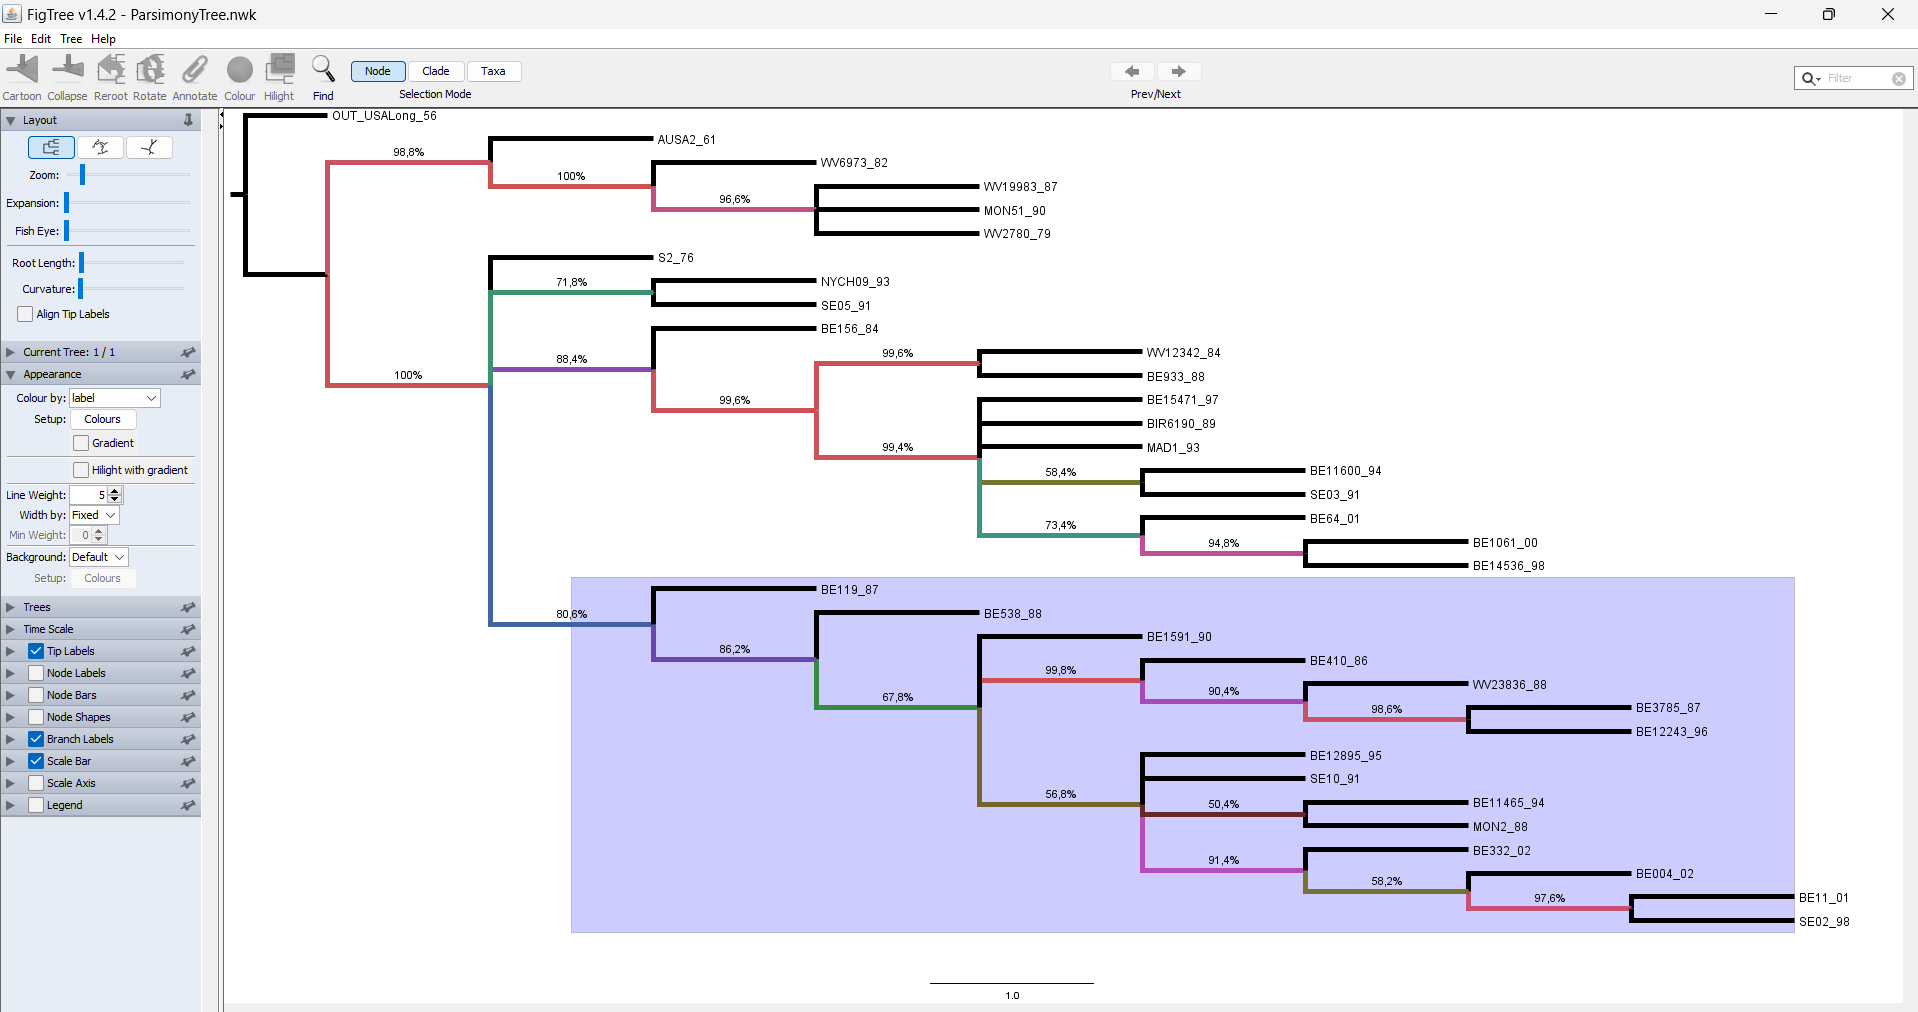
\includegraphics[width = \linewidth]{figs/figtree.png}
\end{figure}

Una de las plataformas para hacer árboles utilizando la máxima parsimonia es \href{https://www.lillo.org.ar/phylogeny/tnt/}{TNT}. El problema es que, pese a ser muy potente, es muy complicado de utilizar.